\graphicspath{{images_low_res/}}

\section{Background of Research}
\label{sec:background}

\subsection{A Comparison of Methods for Screening Strain Fitness }

QFA and SGA are methods for fitness screening using cultures grown on solid agar, both of
which can be performed using a high-throughput protocol (sga ref) \cite{Banks2012}. SGA
uses pinned cultures of higher initial cell density than the dilute liquid cultures used
in QFA. Although SGA allows for more repeats per plate (1536 cultures vs 384 cultures in
QFA), more of the growth curve can be captured with QFA so fits of growth models are more
accurate (see Figure~\ref{fig:qfa_and_sga_growth_curves}) \citep{Lawless2010}.
Comparison of QFA and SGA cultures in Figure~\ref{fig:qfa_and_sga_growth_curves}c shows
how QFA cultures are composed of many individual colonies which increase in thickness,
whereas SGA cultures are composed of a single uniform colony which grows outwards. The
number of individual colonies in a QFA culture is high enough that lag and other
stochastic effects should average out.

Colonyzer \citep{Lawless2010}, a tool for automatic capture of growth curves from images
of both QFA and SGA plates, uses integrated optical density (IOD) as a proxy for cell
density. Figure~\ref{fig:qfa_curves}, courtesy of \citet{Banks2012}, shows an example of
308 growth curves captured by Colonyzer from a QFA plate. In many SGA studies, culture
area, rather than IOD, is used as a proxy for culture density (example
ref). \cite{Lawless2010} found that direct area measurements are more noisy than IOD
measurements and provide a worse fit to the logistic model. To prevent bias in comparison
of data from QFA and SGA we will use Colonyzer to take the more accurate IOD measurements
for both data types.

Fitness screening can also be performed using liquid cultures which are not susceptible to
competition or signalling effects. However, this approach has lower throughput (ref).

\end{multicols}
\graphicspath{{images_low_res/}}
\begin{Figure}
  \centering
  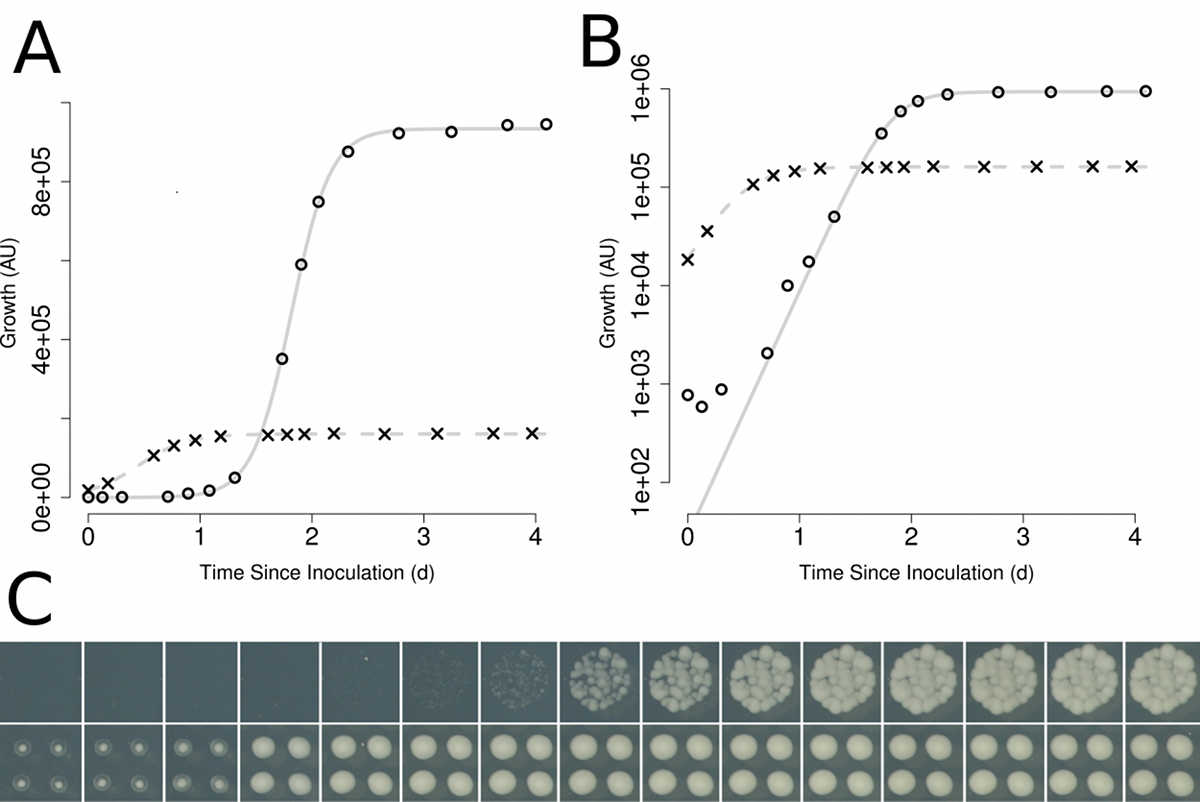
\includegraphics[width=\linewidth]{pin_v_spot_growth}
  \captionof{figure}{Fits of the logistic growth model, to cell density observations of
    yeast growing on solid agar, for spotted cultures (circles) and pinned cultures
    (crosses). In A) culture density is plotted on a linear scale. In B) culture density
    is plotted on a logarithmic scale. C) shows images of the spotted and pinned cultures
    corresponding to the data in A) \& B). Courtesy of \citet{Lawless2010}.}
  \label{fig:qfa_and_sga_growth_curves}
\end{Figure}
\begin{multicols}{2}


\end{multicols}
\graphicspath{{images_low_res/}}
\begin{Figure}
  \centering
  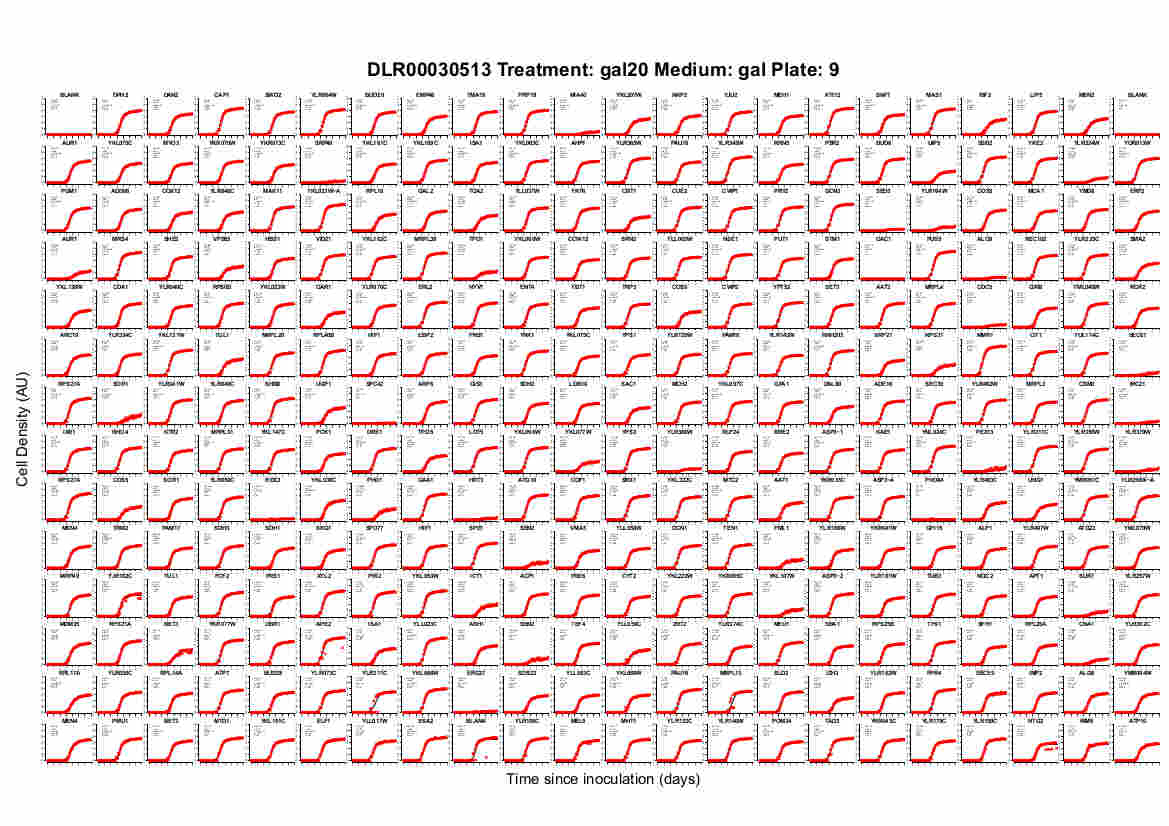
\includegraphics[width=\linewidth]{qfa_growth_array}
  \captionof{figure}{Growth curves, captured automatically by
    Colonyzer \citep{Lawless2010}, of 308 cultures in a QFA
    procedure. Reproduced ??with permission?? from \citet{Banks2012}.}
  \label{fig:qfa_curves}
\end{Figure}
\begin{multicols}{2}


\subsection{Competition and Signalling}

At the beginning of QFA and SGA nutrients are distributed uniformly throughout the
agar. During incubation, cultures grow, consuming nutrients and creating gradients in
nutrient density. A QFA plate taken partway through (at the end of?) incubation can be
seen in Figure~\ref{fig:15_spots}. As some cultures grow much faster than their
neighbours, using more nutrients, we believe that diffusion of nutrients along gradients
between cultures might cause a significant competition effect. Growth of yeast cultures
may also be affected by signal molecules, produced by cultures, which diffuse through the
agar or travel across its surface. Candidates are ethanol \citep{fujita2006}, a poison
produced by fermentation, and chemicals involved in regulatory response
to changes in cell density (quorum sensing) (see \citet{sprague2006,honigberg2011}).

\begin{Figure}
  \centering
  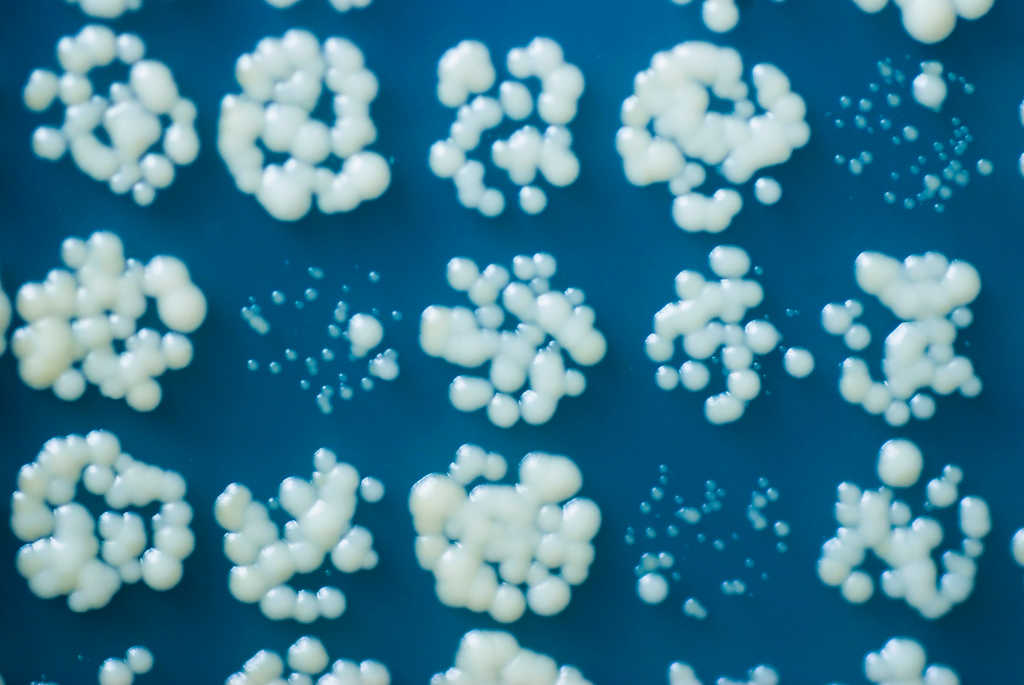
\includegraphics[width=\linewidth]{5658435523_c2e43729f1_b}
  \captionof{figure}{An image of 15 cultures on a section of solid agar from a QFA
    procedure. Image taken with permission from the Colonyzer \citep{Lawless2010} GitHub
    repo https://github.com/CnrLwlss/Colonyzer}
  \label{fig:15_spots}
\end{Figure}

\subsection{Modelling Approaches}

\subsubsection{Mass Action Kinetics}
Chemical reactions are commonly modelled using mass action kinetics, where the rate of a
reaction in a well stirred mixture is proportional to the product of the concentrations of
the reactants. This reflects the probabilistic nature of reactions, which are dependent on
collisions between reactants. If species numbers are large enough, reactions can be
modelled continuously and deterministicly using ordinary differential equations
(ODEs). Microbial population growth, with cell division dependent on nutrient
availability, can also be modelled using mass action kinetics. We can use the following
reaction equation for a culture growing at location \(i\) on an agar,
\begin{subequations}
  \label{eq:9}
  \begin{align}
    &N + C \xrightarrow[]{r_{i}} 2C,\\
    &rate = r_{i}[N][C]
  \end{align}
\end{subequations}
where, \(r_{i}\) is the growth constant, \(C\) is a cell, \(N\) is an amount of nutrients
required for a cell to divide, and [~] are concentrations. In ODE form,
\begin{equation}
  \label{eq:10}
  \frac{dC_{i}}{dt} = r_{i}N_{i}C_{i}
\end{equation}
where \(C_{i}\) and \(N_{i}\) are the amount of cells and nutrients at location \(i\).
The assumption of a well stirred reaction mixture is perhaps not valid for a culture
growing on agar. However, a mass action approximation has been used with some success to
model predator-prey dynamics of animal populations \citep{Berryman1992} and signalling and
reactions in the spatially heterogeneous environment inside cells
\citep{Aldridge2006,Chen2010} where this assumption is also questionable. If nutrient
gradients within cultures are too large then a PDE model may be required. Reactions that
occur at a surface are better modelled using fractal kinetics \citep{savageau1995}.
\subsubsection{The Logistic Growth Model}

The logistic growth model,
\begin{equation}
  \label{eq:1}
  \dot{x} = rx\left(1 - \frac{x}{K}\right)
\end{equation}
\citep{Verhulst1845}, for a population of density \(x\), with parameters, \(r\), growth
rate and \(K\), carrying capacity, describes self-limiting growth and is commonly used
to fit QFA and SGA data with an assumption of independence between cultures. It has the
following analytical solution:
\begin{equation}
  \label{eq:2}
  x(t) = \frac{KPe^{rt}}{K + P(e^{rt}-1)},
\end{equation}
where P is the initial population density. Measures of fitness are commonly defined in
terms of the parameters \(r\), \(K\), and \(P\). For example, \cite{Addinall2011} define two univariate
fitness measures: the maximum doubling rate (MDR) and maximum doubling potential (MDP) as,
\begin{subequations}
  \label{eq:3}
    \begin{align}
      MDR &= \frac{r}{log\left(\frac{2(K-P)}{K-2P}\right)},\\
      MDP &= \frac{log\left(\frac{K}{P}\right)}{log(2)}.
    \end{align}
\end{subequations}
Starting from the mass action kinetic model Lawless (``http://cnr.lwlss.net/DSLMassAction/'')
derives an ODE of equivalent form to \ref{eq:1},
\begin{equation}
  \label{eq:8}
  \frac{dN_{Cell}}{dt} = rN_{Cell}\left(1 - \frac{N_{Cell}}{K}\right),
\end{equation}
where...(maybe don't include this equation explicitly as it could take too much room to
explain?) If we can do this for a mass action kinetic model with competition and
signalling, this will allow us to compare the effect of competition and signalling on
existing fitness measures.

\subsection{Fitness Screening in Functional Genomics}
\label{sec:genetic-interaction}
Fitness screening using cultures grown on solid agar has important uses in functional
genomics for inferring genetic interactions and response to environmental
conditions. \citet{Costanzo2010} use SGA data to construct a genetic interaction map for
\textit{S. cerevisiae} containing \textasciitilde 75\% of the genome. Mutants!

Using QFA and \textit{Saccharomyces cerevisiae}, \citet{Addinall2011} study the genetic
interactions of a mutant \textit{cdc13}, which functions in telomere capping. This offers
a way to discover genes involved in telomere shortening, which is linked to cancer and
ageing, and could lead to health benefits for humans. Important new discoveries could be
made if the power to predict genetic interactions is improved by accounting for
competition and signalling in reanalysis of data from such studies. If competition and
signalling has an affect in yeast this is also likely to be relevant for fitness screening
using other types of microbial organisms.

%%% Local Variables:
%%% mode: latex
%%% TeX-master: "proposal"
%%% End:
